\subsection{Samih Rifat Sergisi}
\begin{wrapfigure}{r}{0.3\textwidth}
    \centering
    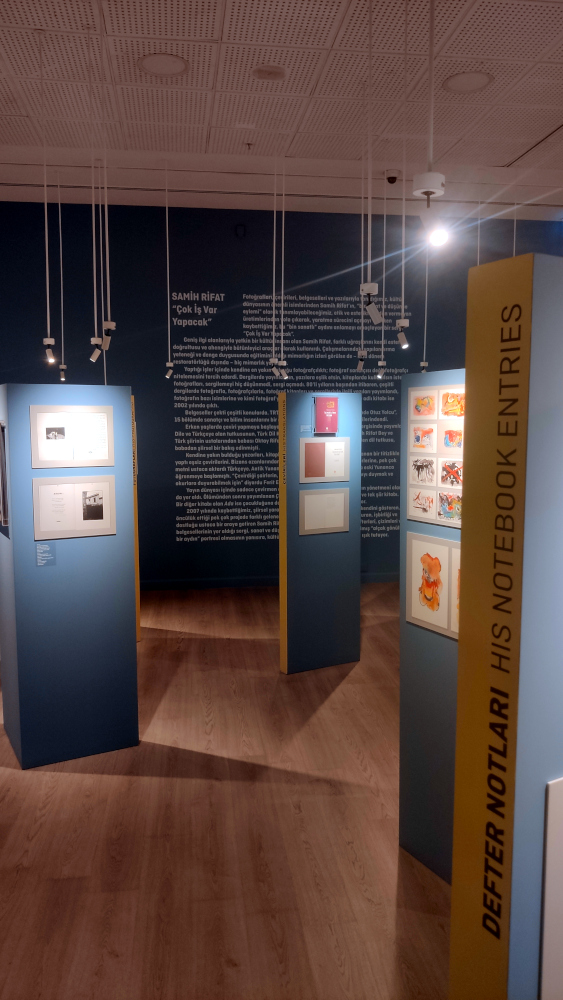
\includegraphics[width=0.25\textwidth]{assets/samih_rifat.jpg}
    \caption{Samih Rifat Sergisi}
\end{wrapfigure}
\indent\indent Samih Rifat, 24 Kasım 1945 tarihinde İstanbul'da doğmuştur. Ünlü şair Oktay Rifat'ın oğludur. İlköğrenimini Beylerbeyi İlkokulu’nda, ortaöğrenimini Saint Benoît Fransız Lisesi’nde tamamlamıştır. Yükseköğrenimini İstanbul Teknik Üniversitesi (İTÜ) Mimarlık Fakültesi’nde tamamlayan Rifat, bir süre kamu kurumlarında mimar olarak görev yapmıştır.\newline
\indent Meslek hayatının ilerleyen dönemlerinde belgesel ve reklam filmi yönetmenliğine yönelmiş; aynı zamanda fotoğrafçılık alanında da üretimlerde bulunmuştur. Üniversite yıllarında başladığı çeviri çalışmalarını 1980’li yıllarda Yazko Çeviri dergisinde yayımlayarak sürdürmüştür. René Char, Jacques Prévert, André Verdet, Jean Follain, Paul Valéry, Vladimir Mayakovski, Konstantinos Kavafis, Amin Maalouf, Yorgos Seferis ve Le Corbusier gibi önemli şair ve yazarlardan Türkçeye çeviriler yapmıştır. Bunlarla beraber, \textit{Aries} ve \textit{Fol} isimlerinde iki dergi yayımlamıştır.\newline
\indent Fotoğrafçılıkla da yakından ilgilenen Samih Rifat, 1980’li yıllardan itibaren çeşitli dergilerde yayımlanan yazılarına kendi fotoğraflarıyla eşlik etmiştir. Bunun yanı sıra, belgesel filmler çekmiş ve müzikle de ilgilenmiştir. Klasik gitar çalan Rifat, 1981 yılında İstanbul Filarmoni Derneği’nin düzenlediği ilk İstanbul Uluslararası Gitar Festivali'nin organizasyonunda görev almış ve festival kapsamında sanatçı Mutlu Torun ile birlikte sahne almıştır.\newline
\indent Müzenin üçüncü katında, 4 Ağustos 2007 tarihinde aramızdan ayrılan Samih Rifat için bir nevi vefa sergisi bulunmaktadır. Sergide Samih Rifat'ın çevirileri, yazıları, yayımladığı dergileri, besteleri, çizimleri ve fotoğraf eserleri bulunmaktadır.